%!TEX root = ../thesis.tex
%*******************************************************************************
%*********************************** Sixth Chapter *****************************
%*******************************************************************************
\chapter{Nonparametric rare event estimation}
%*******************************************************************************
\hfill
\localtableofcontents
\newpage

%============================================================%
%============================================================%
\section{Introduction}
%============================================================%
%============================================================%
Reliability analysis of a system is often associated with rare event probability estimation. 
Considering that the system's performance is modeled by a deterministic scalar function $g: \iD_\bx \subseteq \R^d \rightarrow \R$, called \emph{limit-state function} and a critical threshold on the system's output $\yth\in\R$, one can define the \emph{failure domain} as $\iF_{\bx} := \{\bx \in \iD_\bx | g(\bx) \leq \yth\}$. 
Uncertain inputs are represented by a continuous random vector $\bX \in \iD_\bx$ assumed to be distributed according to its joint probability density function (PDF) $f_\bX$. 
In this context, uncertainty propagation consists in composing the random vector $\bX$ by the function $g$ to get an output variable of interest $Y = g(\bX) \in \R$. 
A usual risk measure in reliability analysis is the \emph{failure probability}, denoted by $\pf$, and defined as the probability that the system exceeds the threshold $\yth$:
%\begin{equation}
%    \pf := \P(g(\bX) \leq \yth)
%        %&= \int_{\iF_\bx} f_\bX(\bx) \, \d\bx\\
%        = \int_{\iD_\bx} \1_{\iF_\bx}(\bx) f_\bX(\bx) \, \d\bx
%\end{equation}
%where $\1_{\iF_\bx}(\cdot)$ is the indicator function of the failure domain such that $\1_{\iF_\bx}(\bx) = 1$ if $\bx \in \iF_\bx$ and $\1_{\iF_\bx}(\bx) = 0$ otherwise. 
Rare event problems are usually solved in the so-called \emph{standard normal space} after applying an ``iso-probabilistic transformation'' which can be either the Rosenblatt or the generalized Nataf one \citep{Lebrun_PHD_2013}.
%VCN : je n'aime pas vraiment cette phrase qui est trop discutable...
%%In structural reliability, a failure probability is considered rare for values between $10^{-2} \leq \pf \leq 10^{-8}$. 
Additionally, the limit-state function $g$ can be viewed as an input-output ``black-box'' model which can be costly to evaluate (e.g., a complex numerical model), making the failure probability estimation nontrivial. 
When the limit-state function is a costly computer model, one can build a surrogate model and use specific active learning methods (see, e.g., \citet{moustapha_ss_2022}). 
However, using surrogate models is not always possible for practical engineering applications as they might introduce another level of approximation, which can be prohibitive from safety auditing. 
Moreover, their validation as well as their behavior with respect to large input dimension case make also their use quite complex (see, e.g.,  \citep{Marrel_Iooss_Chab_ICSCREAM_2020}.

Going back to the rare event estimation literature, one can consider two major types of techniques for failure probability calculation \citep{MorioBalesdent2015}: (i) Geometric approaches, such as the \emph{first-/second-order reliability method} (FORM/SORM) whose aim is to approximate the limit-state function by a first-/second-order Taylor expansion at the most probable failure point; (ii) Simulation-based techniques such as the \emph{crude Monte Carlo} method. 
Unfortunately, FORM/SORM methods do not provide a lot of statistical information as they are purely geometric approaches.
%% VCN : pour moi, ce n'est pas le plus grave. Le plus grave est que ces méthodes ne donennt pas d'info statistique sur l'estimation, car elles relèvent d'un calcul numérique => SORM gère très bien les LSF très courbées !
%fail to solve highly nonlinear or high-dimensional problems
% \citep{Rackwitz_2001}
Meanwhile, estimating a rare event probability by crude Monte Carlo becomes rapidly intractable. 
To overcome this limit, advanced simulation techniques have been developed: among others, one can mention several ``variance reduction methods'' such as the non-adaptive and adaptive versions of the \emph{Importance Sampling} \citep{RubinsteinKroese1981} (either parametric, using the Cross-Entropy method \citet{NKurtz_JSong_StrucSaf_2013}, or nonparametric \citet{Morio_RESS_2011}) and splitting techniques \citep{cerou2012sequential} such as the \emph{Subset Simulation} (SS) \citet{AuBeck2001}. 
In these techniques, the idea is to write the rare event $\pf$ as a product of larger conditional probabilities, each one of them being easier to estimate. 
To generate intermediary conditional samples, this method uses Markov chain Monte Carlo (MCMC) sampling, which presents numerous versions \citep{Papaioannou_PEM_2015}. 
However, MCMC algorithms are known to be highly tunable algorithms which produce non-i.i.d. samples, which consequently, cannot be used for direct statistical estimation (e.g., failure probability or sensitivity indices \citep{daveiga_iooss_2021}. 

% glasserman1999multilevel
% Importance sampling is a variance reduction method used to improve crude Monte Carlo, with various adaptations in the instrumental density construction. Among others, one can refer to the ``adaptive importance sampling by cross-entropy'' \citep{NKurtz_JSong_StrucSaf_2013}, or the ``nonparametric adaptive importance sampling'' \citep{Morio_EJOP_2010}. Alternatively, ``subset sampling'' (SS) \citep{AuBeck2001} (also referred to as ``multilevel splitting'' \citep{glasserman1999multilevel}, or ``sequential Monte Carlo'' \citep{cerou2012sequential}) is a different type of variance reduction method. It constantly relies on the same idea: a rare event can be expressed as a product of nested conditional events (subsets). The failure probability $\pf$ is written as a product of the respective conditional probabilities, each larger than $\pf$ (therefore easier to estimate). To generate intermediary subset samples, this method uses Markov chain Monte Carlo (MCMC) sampling, which presents numerous versions \cite{Papaioannou_PEM_2015}.

The present work proposes a new rare event estimation method, adopting the same sequential structure as SS while using a strictly different sampling mechanism to generate conditional samples. 
This method intends to fit the intermediary conditional distributions with a nonparametric tool called the \emph{Empirical Bernstein Copula}. 
Contrarily to SS, the proposed method named ``Bernstein adaptive nonparametric conditional sampling'' (BANCS), generates i.i.d. samples of the intermediary conditional distributions. 
For instance, a practical use of such i.i.d. samples can be to estimate dedicated reliability-oriented sensitivity indices (see, e.g., \cite{chabridon2021global,marrel_chabridon_2021}).

In this paper, Section 2 will recall the methodology of subset sampling and probabilistic modeling. 
Then, Section 3 will introduce the BANCS method for rare event estimation. 
Section 4 will apply this method to three toy-cases and analyze the results with respect to SS performances. 
Then, the last section present some conclusions and research perspectives.


%============================================================%
\subsection{Background}
%============================================================%

%------------------------------------------------------------%
\subsubsection{Subset sampling}
%------------------------------------------------------------%

Subset sampling splits the failure event $\iF_{\bx}$ into an intersection of $k_\#$ intermediary events $\iF_{\bx} = \cap_{k=1}^{k_\#} \iF_{[k]}$.
Each are nested such that $\iF_{[1]} \supset \dots \supset \iF_{[k_\#]} = \iF_{\bx}$.
The failure probability is then expressed as a product of conditional probabilities:
\begin{equation}
    \pf = \P(\iF_{\bx}) = \P(\cap_{k=1}^{k_\#} \iF_{[k]}) = \prod_{k=1}^{k_\#} \P(\iF_{[k]} | \iF_{[k-1]}).
\end{equation}
From a practical point of view, the analyst tunes the algorithm by setting the intermediary probabilities $\P(\iF_{[k]} | \iF_{[k-1]}) = p_0, \forall k \in \{1, \dots, k_\# \}$. 
Then, the corresponding quantiles $q_{[1]}^{p_0} > \dots > q_{[k_\#]}^{p_0}$ are estimated for each conditional subset samples $\bX_{[k], N}$ of size $N$. 
Note that the initial quantile is estimated by crude Monte Carlo sampling on the input PDF $f_{\bX}$. 
Following conditional subset samples are generated by MCMC sampling of $f_{\bX}(\bx |\iF_{[k-1]})$, using as seeds initialisation points the $n= N p_0$ samples given by $\mathbf{A}_{[k], n}=\{\bX_{[k-1]}^{(j)} \subset \bX_{[k-1], N}| g(\bX_{[k-1]}^{(j)}) > \widehat{q}_{[k-1]}^\alpha \}_{j=1}^n$. 
This process is repeated until an intermediary quantile exceeds the threshold: $\widehat{q}_{[k_\#]}^{p_0} < \yth$. 
Finally, the failure probability is estimated by:
\begin{equation}
    \pf \approx \widehat{\pf}^{\mathrm{SS}} = p_0^{k_\# -1} \frac1N \sum_{j=1}^N \1_{\{g(\bx) \leq \yth\}} (\bX_{[k_\#],N}^{(j)}).
\end{equation}

In practice, the subset sample size should be large enough to properly estimate intermediary quantiles, which leads \cite{AuBeck2001} to recommend setting $p_0=0.1$. SS efficiency depends on the proper choice and tuning of the MCMC algorithm \citep{Papaioannou_PEM_2015}. 
Our work uses the SS implementation from \texttt{OpenTURNS}\footnote{\href{https://openturns.github.io/www/index.html}{https://openturns.github.io/www/index.html}} \citep{baudin_dutfoy_2017} which integrates a component-wise Metropolis-Hastings algorithm. 
As an alternative to generating samples on a conditional distribution by MCMC, one could try to fit this conditional distribution.

%------------------------------------------------------------%
\subsubsection{Multivariate modeling using copulas}
%------------------------------------------------------------%
The  Sklar theorem \citep{joe_1997} affirms that the multivariate distribution of any random vector $\mathbf{X} \in \R^d$ can be broken down into two objects:
\begin{enumerate}
    \item A set of univariate marginal distributions to describe the behavior of the individual variables;
    \item A function describing the dependence structure between all variables, called a copula. 
\end{enumerate}
This theorem states that considering a random vector $\mathbf{X} \in \R^d$, with its distribution $F$ and its marginals $\{F_i\}_{i=1}^d$, there exists a copula $C: [0, 1]^d \rightarrow [0, 1]$, such that:
\begin{equation}
    F(x_1, \dots, x_d) = C\left(F_1(x_1), \dots, F_p(x_d)\right). 
\end{equation}

It allows us to divide the problem of fitting a joint distribution into two independent problems: fitting the marginals and fitting the copula. 
Note that when the joint distribution is continuous, this copula is unique. 
Provided a dataset, this framework allows to combine a parametric (or nonparametric) fit of marginals with a parametric (or nonparametric) fit of the copula. 
When the distribution's dimension is higher than two, one can perform a parametric fit using vine copulas \citep{joe2011dependence}, implying the choice of multiple types of parametric copulas. 
Otherwise, nonparametric fit by multivariate kernel density estimation (KDE) presents a computational burden as soon as the dimension increases \citep{chabridon2021global}. 
Since univariate marginals are usually well-fitted with nonparametric tools (e.g., KDE), let us introduce an effective nonparametric method for copula fitting.


%============================================================%
%============================================================%
\section{Bernstein adaptive nonparametric conditional sampling}
%============================================================%
%============================================================%

%------------------------------------------------------------%
\subsection{Empirical Bernstein copula}
%------------------------------------------------------------%

Copulas are continuous and bounded functions defined on a compact set (the unit hypercube). 
Bernstein polynomials allow to uniformly approximate as closely as desired any continuous and real-valued function defined on a compact set (Weierstrass approximation theorem). 
Therefore, they are good candidates to approximate unknown copulas. 
This concept was introduced as \emph{empirical Bernstein copula} (EBC) by \cite{sancetta_satchell_2004} for applications in economics and risk management. 
Later on, \cite{segers_2017} offered further asymptotic studies. 
Formally, the multivariate Bernstein polynomial for a function $C: [0, 1]^d \rightarrow \R$ on a grid over the unit hypercube $G:=\left\{\frac{0}{m_1}, \dots, \frac{m_1}{m_1}\right\} \times \dots \times \left\{\frac{0}{m_d}, \dots, \frac{m_d}{m_d}\right\}, \bm = (m_1, \dots, m_d) \in \N^d$, writes: 
\begin{equation}
    B_{\bm}(C)(\bu) := \sum_{t_1=0}^{m_1} \dots \sum_{t_d=0}^{m_d} C\left(\frac{t_1}{m_1}, \dots, \frac{t_d}{m_d}\right) \prod_{j=1}^d P_{m_j, t_j}(u_j),\label{eq:ebc}
\end{equation}
with $\bu = (u_1, \dots, u_d) \in [0, 1]^d$, and the Bernstein polynomial $P_{m, t}(u):= \frac{t!}{m!(t-m)!}u^m(1-u)^{t-m}$. 
Notice how the grid definition implies the polynomial's order. 
When $C$ is a copula, then $B_{\bm}(C)$ is called ``Bernstein copula''. 
Therefore, the empirical Bernstein copula is an application of the Bernstein polynomial in \eq{eq:ebc} to the so-called ``empirical copula''.

In practice, considering a sample $\bX_n = \left\{\bx^{(1)}, \dots, \bx^{(n)}\right\} \in \R^{np}$ and the associated ranked sample $\bR_n = \left\{\br^{(1)}, \dots, \br^{(n)}\right\}$, the corresponding empirical copula writes: 
\begin{equation}
    C_n(\bu) := \frac1n \sum_{i=0}^{n} \prod_{j=1}^{p} \1 \left\{ \frac{r_j^{(i)}}{n} \leq u_j \right\},
\end{equation}
with $\bu = (u_1, \dots, u_d) \in [0, 1]^d$. In the following, the polynomial order is set as equal in each dimension: $\{m_i = m\}_{j=1}^d$. 
Theoretically, the tuning parameter can be optimized to minimize an ``Mean Integrated Squared Error'' (MISE), leading to a bias-variance tradeoff. 
Formally, the MISE of the empirical Bernstein copula $B_{\bm}(C_n)$ is defined as follows:
\begin{equation}
    \E\!\left[ \lVert B_{\bm}(C_n) - C \rVert^2_2 \right] \!=\! \E\!\left[\!\int_{\R^d}\! \left(B_{\bm}(C_n)(\bu) \!-\! C(\bu) \d \bu \right)^2 \!\right]\!\!.
    \label{eq:kimse}
\end{equation}
Then, \cite{sancetta_satchell_2004} prove in their Theorem 3 that: 
\begin{itemize}
    \item $B_{\bm}(C_n)(\bu) \rightarrow C(\bu)$ for any $u_j \in \left]0, 1\right[$ if $\frac{m^{d/2}}{n} \rightarrow 0$, when $m, n \rightarrow \infty$.
    \item The optimal order of the polynomial in terms of MISE is: $m \lesssim m_{\mathrm{IMSE}} = n^{2/(d+4)}, \forall u_j \in \left]0, 1\right[$. The sign $\lesssim$ means ``less than or approximately''.
\end{itemize}

Let us remark that in the special case $m = n$, also called the ``Beta copula'' in \cite{segers_2017}, the bias is very small while the variance gets large. 
To illustrate the previous theorem, \cite{lasserre_2022} represents the evolution of the $m_{\mathrm{IMSE}}$ for different dimensions and sample sizes (see \fig{fig:hmise}). 
In high dimension, the values of $m_{\mathrm{IMSE}}$ tend towards one, which is equivalent to the independent copula. 
Therefore, high-dimensional problems should be divided into a product of smaller problems on which the EBC is tractable. 
Provided a large enough learning set $\bX_n$, KDE fitting of marginals combined with EBC fitting of the copula delivers good results even on complex dependence structures. 
Moreover, EBC provides an explicit expression, making a Monte Carlo generation of i.i.d. samples simple. 
In the following, this nonparametric tool is used to fit the intermediary conditional distributions present in subset sampling.  

\begin{figure}
    \centering
    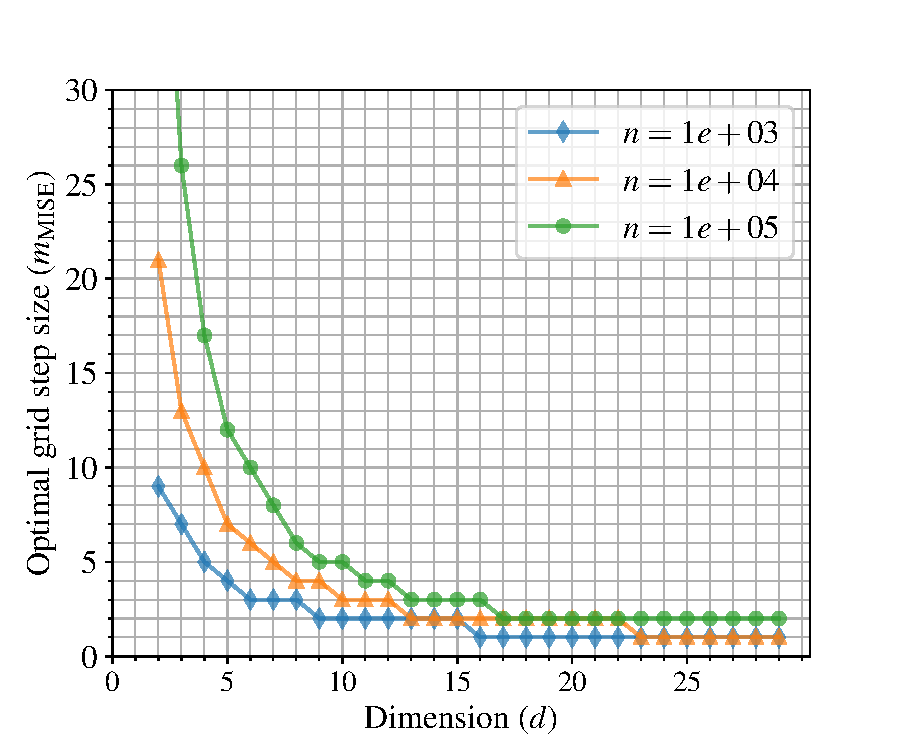
\includegraphics[width=0.6\linewidth]{part3/figures/BANCS/hMISE.pdf}
    \caption{Evolution of $m_{\mathrm{IMSE}}$ for different dimensions and sample sizes.}
    \label{fig:hmise}
\end{figure}


%------------------------------------------------------------%
\subsection{Bernstein adaptive nonparametric conditional sampling algorithm}
%------------------------------------------------------------%

This new method reuses the main idea from SS while employing a different approach to generate conditional samples. 
Instead of using MCMC sampling, the conditional distribution is firstly fitted by a nonparametric procedure, before sampling on this nonparametric model. 
As described in Algorithm \ref{alg:bancs}, conditional sampling is done on a distribution composed by merging marginals $\{\widehat{F}_i\}_{i=1}^d$ fitted by KDE, with a copula  $B_\bm(C_n)$ fitted by EBC. 
\fig{fig:bancs_illustration1} illustrate the nonparametric fit and conditional sampling in BANCS method on a two-dimensional reliability problem (later introduced as ``toy-case \#1''). 
At iteration $k$, after estimating the intermediary quantile $\widehat{q}_{[k]}^{p_0}$, a nonparametric model is fitted on $\mathbf{A}_{[k+1], n}$ and used to generate the next $N$-sized subset sample $\bX_{[k+1], N}$. 
Note that the BANCS method does not require iso-probabilistic transform.

%%%%%%%%%%%%%%%%%%%%%%%%%%%%%%%%%%%%%%%%%%%%%%%%%%%%%%%%%%%%%
\begin{algorithm}[h]
\caption{Bernstein adaptive nonparametric conditional sampling (BANCS).}\label{alg:bancs}
\footnotesize
\begin{algorithmic}
\LComment{Inputs:}
\State $f_\bX$, joint PDF of the inputs
\State $g(\cdot)$, limit-state function
\State $\yth \in \R$, threshold defining the failure event 
\State $N$, number of samples per iteration
\State $m \in \N$, parameter of the EBC fitting
\State $p_0 \in \left]0, 1\right[$, empirical quantile order (rarity parameter)
\LComment{Algorithm:}
\State Set $k = 0$ and $f_{[0]} = f_\bX$
\State Sample $\bX_{[0], N} = \{\bX_{[0]}^{(j)}\}_{j=1}^N \overset{\text{i.i.d}}{\sim} f_{[0]}$
\State Evaluate $G_{[0], N} = \{g(\bX_{[0]}^{(j)})\}_{j=1}^N$
\State Estimate the empirical $p_0$-quantile $\widehat{q}_{[0]}^{p_0}$ of the set $G_{[0], N}$

\While{$\widehat{q}_{[k]}^{p_0} > \yth$}
\State Subsample $\mathbf{A}_{[k+1], n}=\{\bX_{[k]}^{(j)} \subset \bX_{[k], N}| g(\bX_{[k]}^{(j)}) > \widehat{q}_{[k]}^{p_0} \}_{j=1}^n$
\State Fit marginals of the subset $\mathbf{A}_{[k+1], n}$ by KDE $\{\widehat{F}_i\}_{i=1}^d$
\State Fit the copula of the subset $\mathbf{A}_{[k+1], n}$ by EBC $B_\bm(C_n)$
\State Build a CDF $\widehat{F}_{[k+1]}(\bx) = B_\bm(C_n)(\widehat{F}_1(x_1), \dots, \widehat{F}_d(x_d))$
\State Sample $\bX_{[k+1], N} = \{\bX_{[k+1]}^{(j)}\}_{j=1}^N \overset{\text{i.i.d}}{\sim} \widehat{f}_{[k+1]}$
\State Evaluate $G_{[k+1], N} = \{g(\bX_{[k+1]}^{(j)})\}_{j=1}^N$
\State Estimate the empirical $p_0$-quantile $\widehat{q}_{[k+1]}^{p_0}$ of $G_{[k+1], N}$
\State Set $k = k+1$
\EndWhile
\State Set total iteration number $k_\# = k-1$ 
\State Estimate $\widehat{\pf} = (1 - p_0)^{k_\#} \cdot \frac{1}{N} \sum_{j=1}^N \1_{\{g(\bX_{[k_\#]}^{(j)}) \geq \yth  \}}(\bX_{[k_\#]^{(j)}}) $
\LComment{Outputs:}
\State $\widehat{\pf}$, estimate of $\pf$
\end{algorithmic}
\end{algorithm}
%%%%%%%%%%%%%%%%%%%%%%%%%%%%%%%%%%%%%%%%%%%%%%%%%%%%%%%%%%%%%

\begin{figure}[!ht]
    \centering
    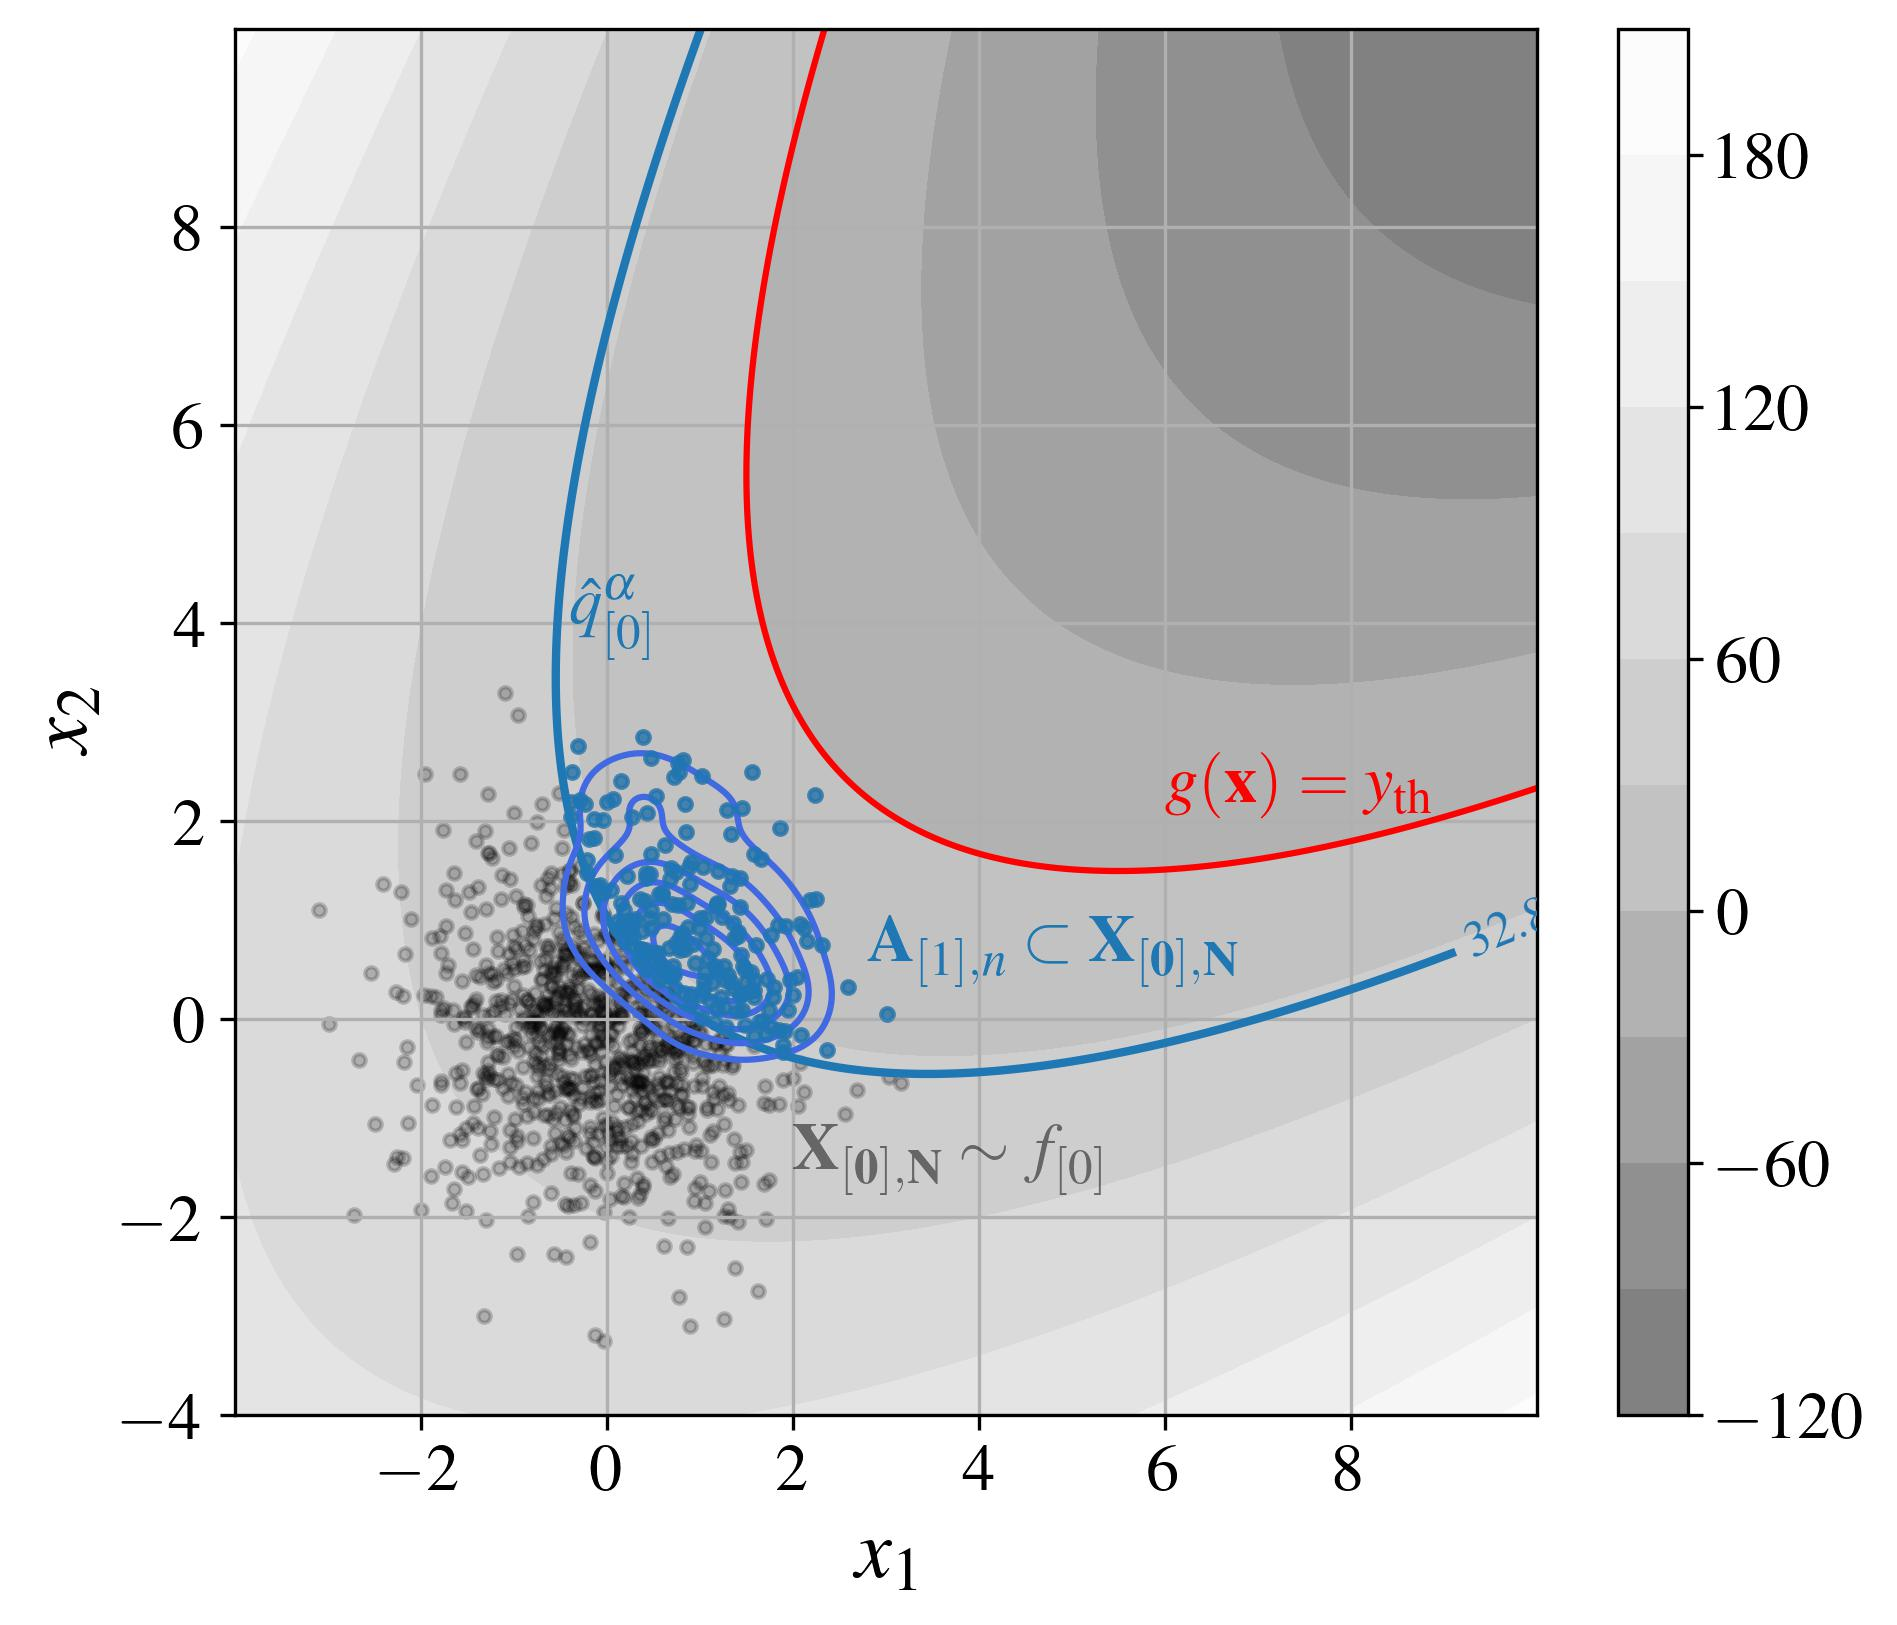
\includegraphics[width=0.48\linewidth]{part3/figures/BANCS/bancs_illustration1.jpg}
    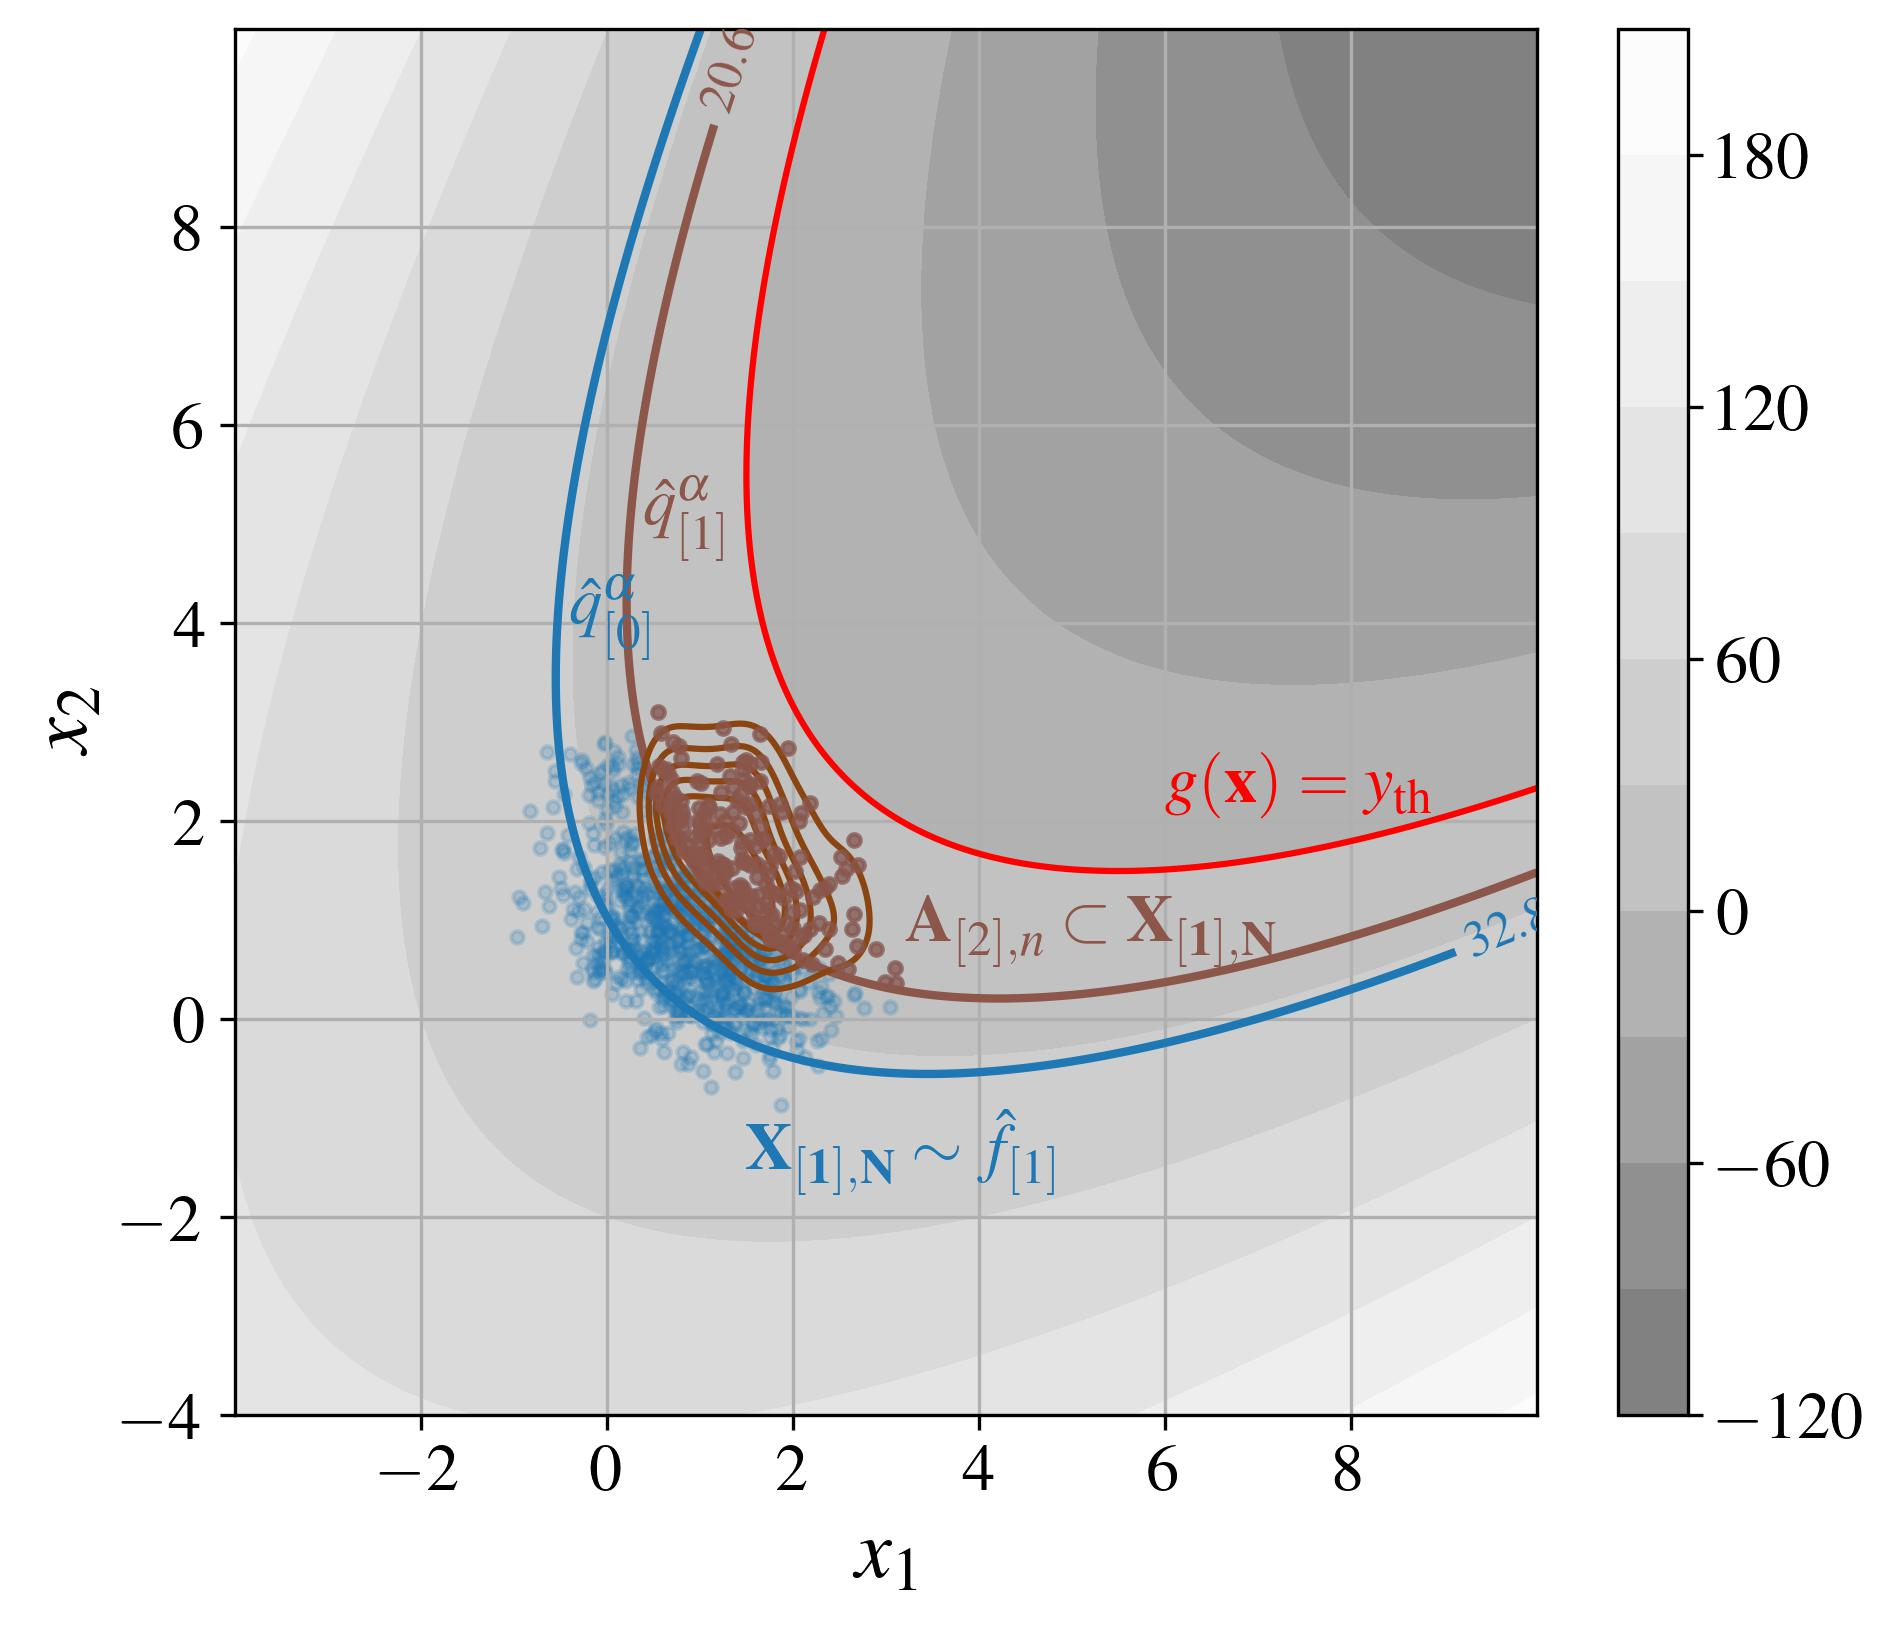
\includegraphics[width=0.48\linewidth]{part3/figures/BANCS/bancs_illustration2.jpg}
    \caption{BANCS on toy-case \#1: illustration of conditional sampling and nonparametric fit at the first and second iterations.}
    \label{fig:bancs_illustration1}
\end{figure}
%%%%%%%%%%%%%%%%%%%%%%%%%%%%%%%%%%%%%%%%%%%%%%%%%%%%%%%%%%%%%

As discussed in the previous section, EBC fitting is tuned by the Bernstein polynomial of order $m$, implying a bias-variance tread off. 
In \fig{fig:bancs_illustration1}, conditional distributions fitted by EBC (blue and brown isolines) seem to present a slight bias since they overlay the quantiles. 
However, reducing this bias implies decreasing the tuning parameter $m$, until $m=1$, which is equivalent to an independent copula. 
Tools to control the goodness of fit of nonparametric conditional distributions are also available. 
As an example, let us consider the fitted conditional distribution at the first iteration (visible in \fig{fig:bancs_illustration1}). 
Its quantile-quantile plot in \fig{fig:qqplot} shows a good fit of the two marginals by KDE. 
Then, the goodness of fit of copulas can be evaluated by Kendall's plot, represented in \fig{fig:kendall_plot}. 
This fit is also good, even if a slight bias is again visible.

\begin{figure}[!ht]
    \centering
    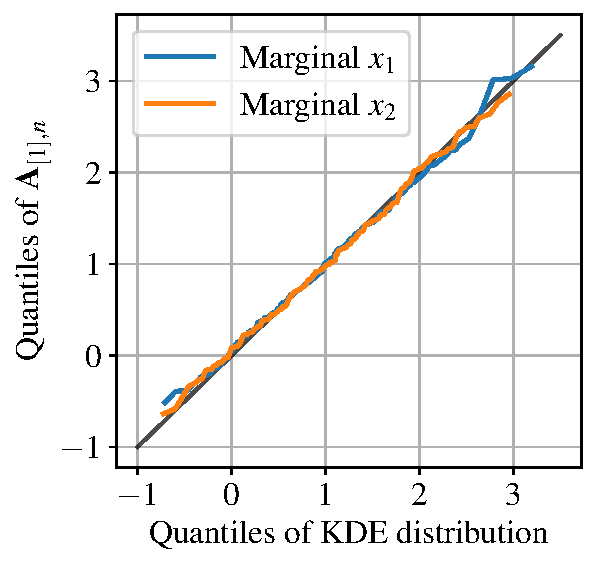
\includegraphics[width=0.6\linewidth]{part3/figures/BANCS/qqplots.pdf}
    \caption{QQ-plot for KDE of marginals of the conditional distribution from \fig{fig:bancs_illustration1}.}
    \label{fig:qqplot}
\end{figure}

\begin{figure}[!ht]
    \centering
    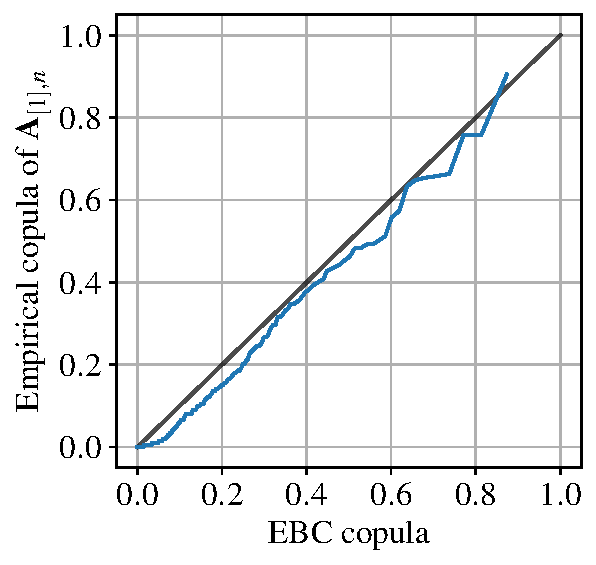
\includegraphics[width=0.6\linewidth]{part3/figures/BANCS/kendall_plot.pdf}
    \caption{Kendall plot for EBC on the copula of a conditional distribution from \fig{fig:bancs_illustration1}.}
    \label{fig:kendall_plot}
\end{figure}


%============================================================%
%============================================================%
\section{Numerical experiments}
%============================================================%
%============================================================%
In the following analytical numerical experiments, the intermediary probabilities were set to $p_0=0.1$, allowing a fair comparison with subset sampling. 
Then, the subset sample size is set to $N=10^4$, in order to get a reasonable sample size $n = N p_0 = 10^3$ to perform the nonparametric fitting. 
EBC tuning is setup to minimize the MISE in \eq{eq:kimse}: $m = 1 + n^{\frac{2}{d+4}}$. 
In order to take into account the variability of the method's results, each experiment is repeated 100 times, allowing the computation of a coefficient of variation $\widehat{\delta} = \frac{\sigma_{\widehat{\pf}}}{\mu_{\widehat{\pf}}}$. 
Note that an implementation of the BANCS method and the following numerical experiments are available in a Git repository\footnote{\url{https://github.com/efekhari27/icasp14}}. 

%------------------------------------------------------------%
\paragraph{Toy-case \#1: Parabolic reliability problem}
%------------------------------------------------------------%

Let us define the parabolic reliability problem, considering the function $g_1: \R^2 \rightarrow \R$:
\begin{equation}
    g_1(\bx)= (x_1 - x_2) ^ 2 - 8 (x_1 + x_2 - 5),
\end{equation}
with the input random vector $\bX = (X_1, X_2)$ following a standard 2-dimensional normal distribution. 
The reliability problem consists in evaluating: $p_{\mathrm{f}, 1} = \mathbb{P} ( g_1(\bX) \leq 0 ) = 1.31 \times 10^{-4}$.

%------------------------------------------------------------%
\paragraph{Toy-case \#2: Four-branch reliability problem}
%------------------------------------------------------------%

Let us define the four-branch reliability problem (originally proposed by \cite{waarts2000structural}), considering the following function $g_2: \R^2 \rightarrow \R$:
\begin{align}
  g_2(\bx) = \min \begin{pmatrix}
    5+0.1(x_1-x_2)^2-\frac{(x_1+x_2)}{\sqrt{2}}\\
    5+0.1(x_1-x_2)^2+\frac{(x_1+x_2)}{\sqrt{2}}\\
    (x_1-x_2)+ \frac{9}{\sqrt{2}}\\
    (x_2-x_1)+ \frac{9}{\sqrt{2}}
  \end{pmatrix},
\end{align}
with the input random vector $\bX = (X_1, X_2)$ following a standard 2-dimensional normal distribution. 
The reliability problem consists in evaluating: $p_{\mathrm{f}, 2} = \mathbb{P} ( g_2(\bX) \leq 0 ) =  2.21 \times 10^{-4}$.

%------------------------------------------------------------%
\paragraph{Toy-case \#3: high-dimensional reliability problem}
%------------------------------------------------------------%

Let us define the higher-dimensional reliability problem (proposed by \cite{yun2018efficient}), considering the following function $g_3 : \R^7 \rightarrow \R$:

\begin{equation}
    g_3(\bx) = 15.59 \times 10^4 - \frac{x_1 x_3^2}{2 x_3^2} \frac{x_2^4 - 4 x_5 x_6 x_7^2 + x_4 (x_6 + 4 x_5 + 2 x_6 x_7)}{x_4 x_5 (x_4 + x_6 + 2 x_6 x_7)},
\end{equation}
with the input random vector $\bX = (X_1, \dots, X_7)$, following a product of normal distributions defined in \cite{yun2018efficient}. 
The reliability problem consists in evaluating: $p_{\mathrm{f}, 3} = \mathbb{P} ( g_3(\bX) \leq 0 ) =  8.10 \times 10^{-3}$.


%------------------------------------------------------------%
\subsection{Results analysis}
%------------------------------------------------------------%

Results of our numerical experiments are presented graphically (for 2-dimensional problems) in Figures  \ref{fig:toycase1_reliability} and \ref{fig:toycase2_reliability}, and numerically in Table \ref{tab:result_table}. 
In the same fashion as the previous illustrations, the figures represent the intermediary quantiles $\widehat{q}_{[k]}^{p_0}$ estimated over conditional samples of size $N=10^4$. 
Moreover, samples $\mathbf{A}_{[k+1], n}$ exceeding these quantiles are also represented in the same color. 
Notice how the last estimated quantile is set to the problem threshold $\yth = 0$. 
To capture the dispersion of BANCS estimation, 100 repetitions were realized. 
Let us notice that for each toy-case, BANCS well estimates the failure probabilities' orders of magnitude. 
Yet the numerical values in Table \ref{tab:result_table} consistently present a positive bias, leading to an overestimated failure probability. 
This bias is partially explained by the EBC tuning choice and could be reduced at the expense of a slightly higher variance.

The variance obtained with the repetitions is quite large. 
Although, part of it is due to the fact that the algorithm might compute a different total number of subsets (e.g., toy-case \#1 is either solved in four or five subsets). 
Overall, considering the EBC tuning from \eq{eq:kimse}, BANCS performs worst than SS on toy-cases \#1 and \#2 but performs as well as SS on the toy-case \#3. 
This might be due to the fact that toy-case \#3 has a higher input dimension. 
However, one can note that SS coefficient of variation is computed by an approximation, tending to underestimate the true coefficient of variation (see e.g., \cite{Papaioannou_PEM_2015}). 

\begin{figure}
    \centering
    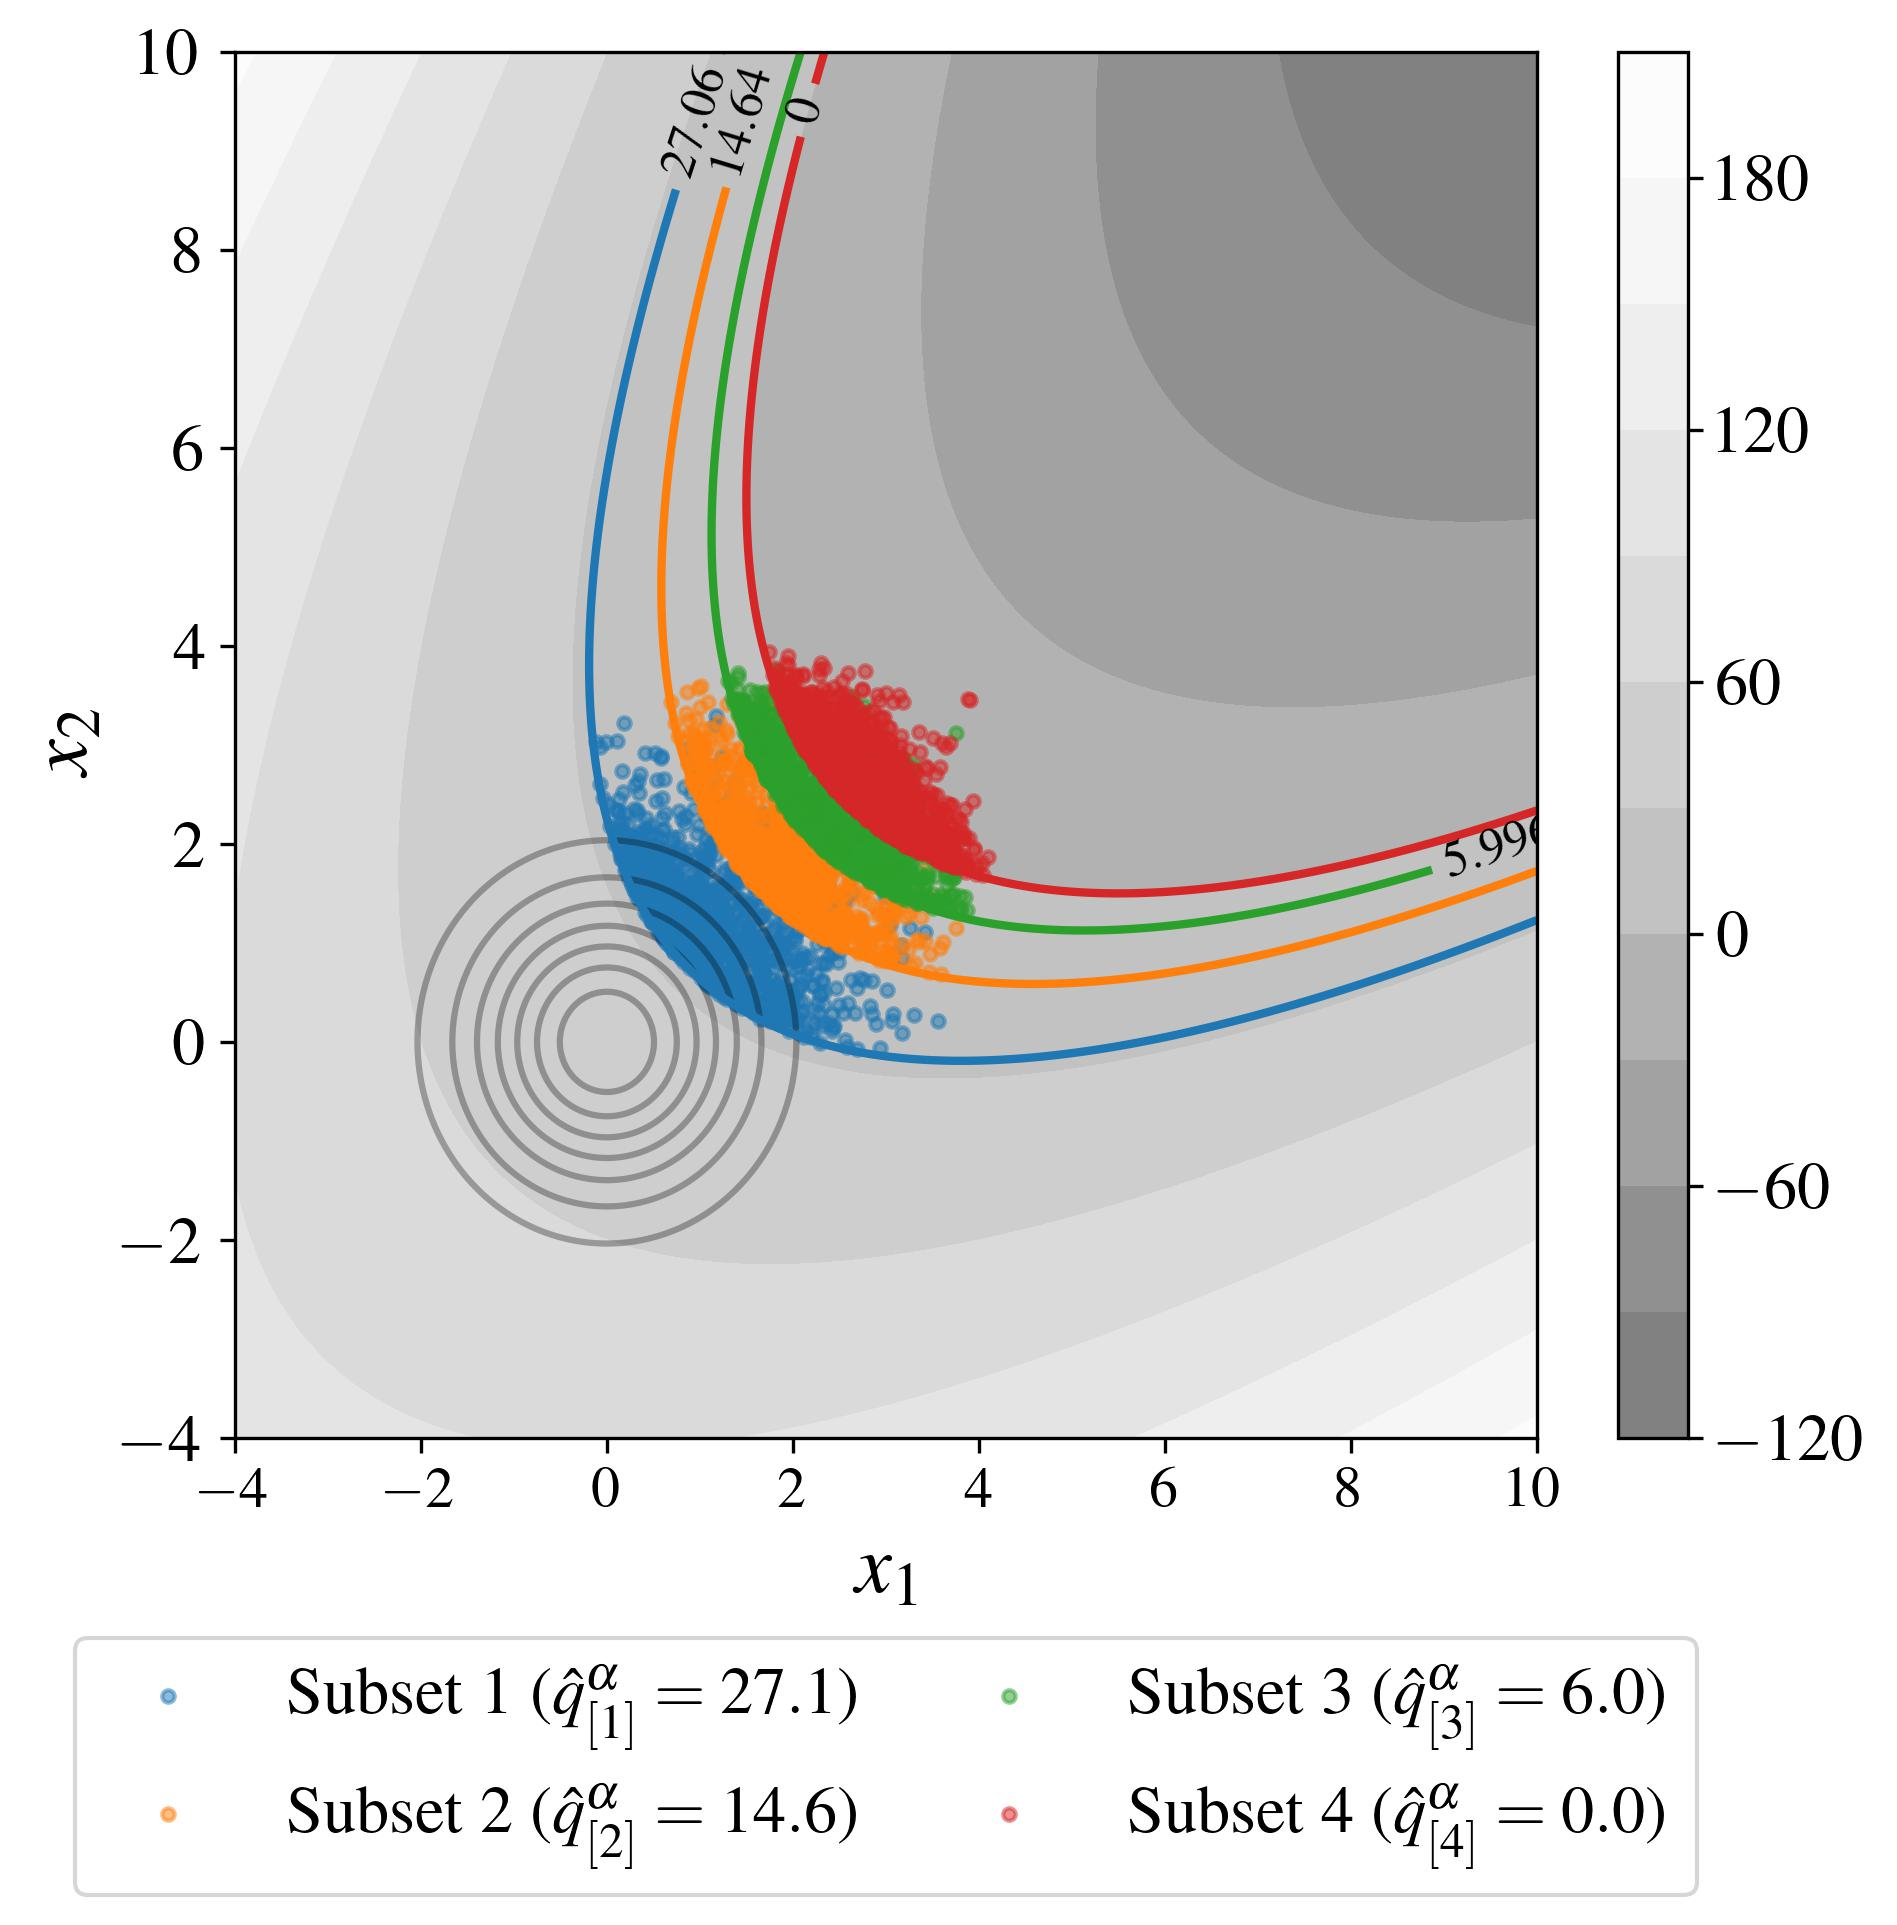
\includegraphics[width=0.6\linewidth]{part3/figures/BANCS/bancs_parabolic2.jpg}
    \caption{BANCS sampling steps on toy-case \#1.}
    \label{fig:toycase1_reliability}
\end{figure}

\begin{figure}
    \centering
    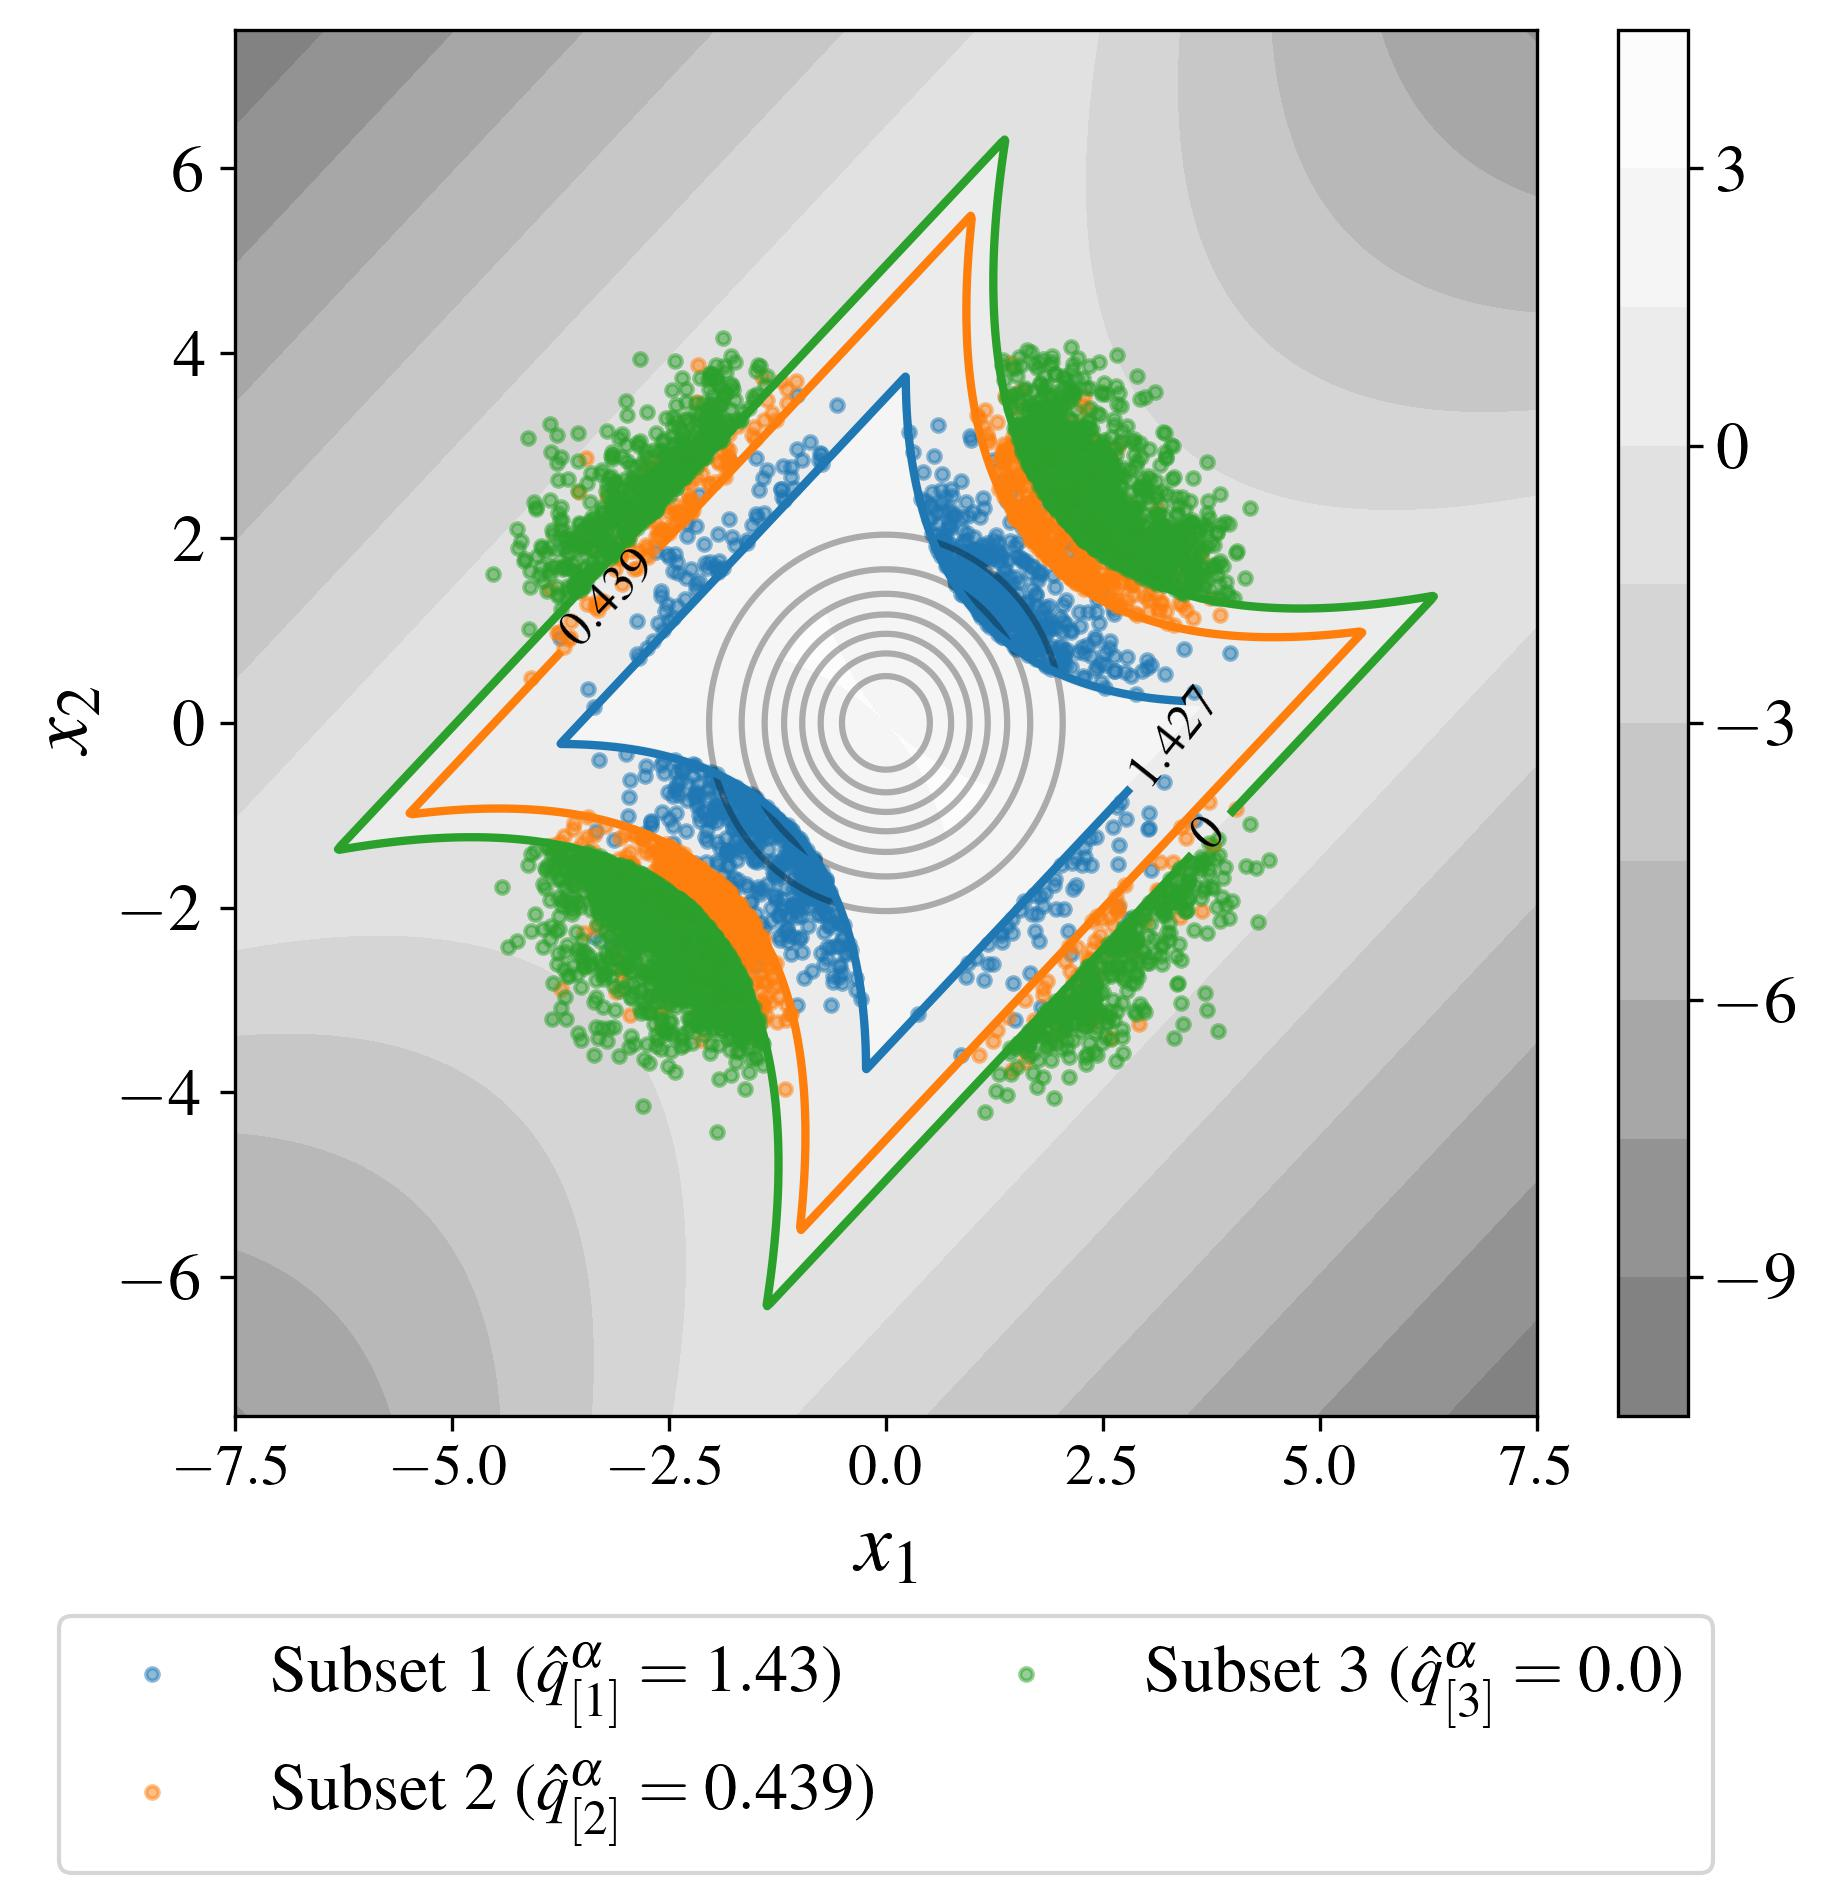
\includegraphics[width=0.6\linewidth]{part3/figures/BANCS/bancs_4branch.jpg}
    \caption{BANCS sampling steps on toy-case \#2.}
    \label{fig:toycase2_reliability}
\end{figure}

%%%%%%%%%%%%%%%%%%%%%%%%%%%%%%%%%%%%%%%%%%%%%%%%%%%%%%%%%%%%%%%
\begin{table*}[h]
    \centering
    \caption{Results of the numerical experiments (subset sample size $N=10^4$, $p_0=0.1$).}
    \begin{tabular}{|l|l|l||l|l||l|l|}\hline
     & $d$ & $\pf^{\mathrm{ref}}$ & $\widehat{\pf}^{\mathrm{BANCS}}$ & $\widehat{\delta}^{\mathrm{BANCS}}$ & $\widehat{\pf}^{\mathrm{SS}}$ & $\widehat{\delta}^{\mathrm{SS}}$\\
    \hline
    Toy-case \#1 & 2 & $1.31 \times 10^{-4}$ & $2.67 \times 10^{-4}$ & $24 \%$ & $1.30 \times 10^{-4}$ & $9 \%$\\
    \hline
    Toy-case \#2 & 2 & $2.21 \times 10^{-4}$ & $4.23 \times 10^{-4}$ & $7 \%$ & $2.24 \times 10^{-4}$ & $6 \%$\\
    \hline
    Toy-case \#3 & 7 & $8.10 \times 10^{-3}$ & $9.32 \times 10^{-3}$ & $15 \%$ & $8.92 \times 10^{-3}$ & $6 \%$\\ \hline
    \end{tabular}
    \label{tab:result_table}
\end{table*}



\section{Application to wind turbine fatigue reliability}
%\section{Application to a floating offshore wind turbine reliability}

%============================================================%
%============================================================%
\section{Conclusion}
%============================================================%
%============================================================%
Subset Simulation uses MCMC sampling to generate its intermediary conditional samples. 
However, MCMC algorithms tends to be complex to tune and does not generate i.i.d. conditional samples. 
In this work, a new method is proposed, replacing MCMC sampling with a simpler procedure. 
An intermediary conditional distribution is first fitted by a nonparametric approach, mixing kernel density estimation for fitting the marginals and Empirical Bernstein Copula (EBC) for fitting the copula. 
Then, the resulting allows to perform direct Monte Carlo sampling. 
This method is named ``Bernstein adaptive nonparametric conditional sampling'' (BANCS) and is applied to three toy-cases (two 2-dimensional and one 7-dimensional) and compared with SS.

The method shows promising results, even though a small positive bias consistently appears. 
This issue results from EBC tuning, creating a bias-variance tradeoff in the copula fit. 
Theoretical works offer optimal tuning, allowing us to find the optimal compromise. 
In our numerical experiments, an empirical estimation of BANCS variance is computed over a set of repetitions. 
BANCS estimated coefficient of variation is higher than SS approximated coefficient of variation. 
This work can be further explored by building an approximation of BANCS variance and confidence interval. 
One major advantage remains that the samples generated at each iteration are i.i.d. leading to a possible use of these samples to perform global reliability-oriented sensitivity analysis \citep{marrel_chabridon_2021} 
in order to detect and analyze the most influential input variables leading to failure.